\documentclass{article}
\usepackage[paperwidth=9.6cm,paperheight=11.2cm,margin=0.35cm]{geometry}
\usepackage{tikz}
\usetikzlibrary{shapes.geometric, arrows.meta, positioning, calc}

\definecolor{navy}{RGB}{15, 23, 42}
\definecolor{borderblue}{RGB}{59, 130, 246}
\definecolor{processblue}{RGB}{239, 246, 255}
\definecolor{tealbg}{RGB}{240, 253, 250}
\definecolor{tealborder}{RGB}{13, 148, 136}
\definecolor{purplebg}{RGB}{250, 245, 255}
\definecolor{purpleborder}{RGB}{147, 51, 234}
\definecolor{amberbg}{RGB}{254, 243, 199}
\definecolor{amberborder}{RGB}{217, 119, 6}
\definecolor{rosebg}{RGB}{255, 241, 242}
\definecolor{roseborder}{RGB}{225, 29, 72}

\tikzset{
    startstop/.style={
        rectangle, rounded corners=7pt, minimum width=2.4cm, minimum height=0.48cm,
        text centered, draw=navy, fill=navy, text=white, font=\bfseries\scriptsize,
        inner sep=2pt
    },
    block/.style={
        rectangle, rounded corners=4pt, minimum width=8.6cm, minimum height=0.52cm,
        text width=8.3cm, text centered, draw=borderblue, fill=processblue,
        font=\scriptsize\bfseries, line width=0.8pt, inner sep=3pt
    },
    blocksplit/.style={
        rectangle, rounded corners=4pt, minimum width=4.1cm, minimum height=0.68cm,
        text width=3.9cm, text centered, font=\scriptsize\bfseries, line width=0.8pt, inner sep=2pt
    },
    arrow/.style={
        thick, -{Stealth[length=4pt, width=3pt]}, draw=navy!85, line width=0.9pt
    }
}

\begin{document}
\thispagestyle{empty}
\centering
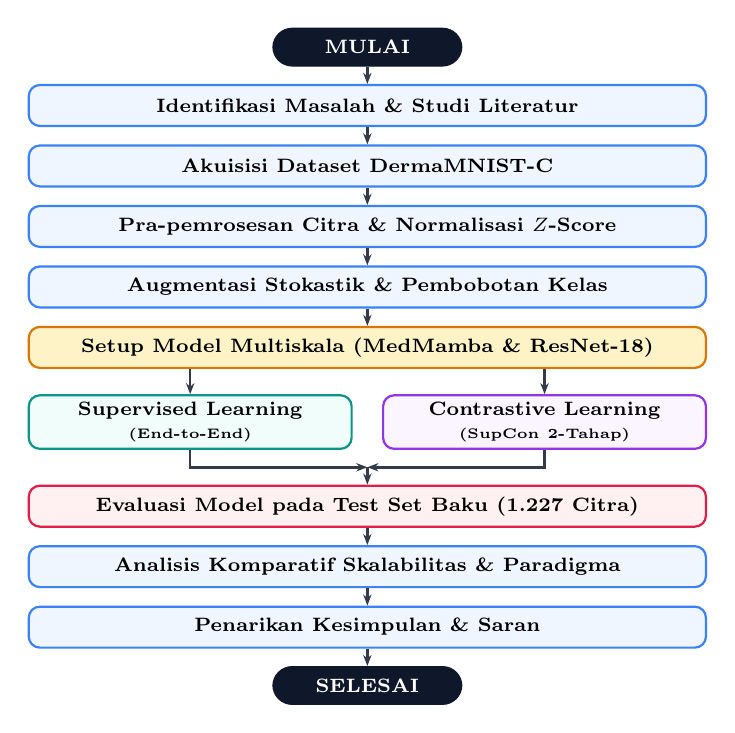
\begin{tikzpicture}[node distance=0.22cm, auto]

    % 1. Start
    \node (start) [startstop] {MULAI};

    % 2. Identifikasi & Studi Literatur
    \node (prob) [block, below = of start] {Identifikasi Masalah \& Studi Literatur};

    % 3. Akuisisi Data
    \node (data) [block, below = of prob] {Akuisisi Dataset DermaMNIST-C};

    % 4. Preprocessing
    \node (prep) [block, below = of data] {Pra-pemrosesan Citra \& Normalisasi $Z$-Score};

    % 5. Augmentasi & CWCE
    \node (aug) [block, below = of prep] {Augmentasi Stokastik \& Pembobotan Kelas};

    % 6. Setup Model
    \node (models) [block, below = of aug, fill=amberbg, draw=amberborder] {Setup Model Multiskala (MedMamba \& ResNet-18)};

    % 7. Paradigma 1 vs 2
    \node (para1) [blocksplit, fill=tealbg, draw=tealborder, anchor=north] at ($(models.south) + (-2.25cm, -0.32cm)$) {
        Supervised Learning\\{\tiny (End-to-End)}
    };

    \node (para2) [blocksplit, fill=purplebg, draw=purpleborder, anchor=north] at ($(models.south) + (+2.25cm, -0.32cm)$) {
        Contrastive Learning\\{\tiny (SupCon 2-Tahap)}
    };

    \coordinate (merge) at ($(para1.south)!0.5!(para2.south) - (0, 0.22cm)$);

    % 8. Evaluasi
    \node (eval) [block, below = 0.22cm of merge, fill=rosebg, draw=roseborder] {Evaluasi Model pada Test Set Baku (1.227 Citra)};

    % 9. Analisis
    \node (analysis) [block, below = of eval] {Analisis Komparatif Skalabilitas \& Paradigma};

    % 10. Kesimpulan
    \node (concl) [block, below = of analysis] {Penarikan Kesimpulan \& Saran};

    % 11. Selesai
    \node (end) [startstop, below = of concl] {SELESAI};

    % Connections
    \draw [arrow] (start) -- (prob);
    \draw [arrow] (prob) -- (data);
    \draw [arrow] (data) -- (prep);
    \draw [arrow] (prep) -- (aug);
    \draw [arrow] (aug) -- (models);

    % Branching to Paradigms
    \draw [arrow] ($(models.south) + (-2.25cm, 0)$) -- (para1.north);
    \draw [arrow] ($(models.south) + (+2.25cm, 0)$) -- (para2.north);

    % Merging from Paradigms
    \draw [arrow] (para1.south) |- (merge);
    \draw [arrow] (para2.south) |- (merge);
    \draw [arrow] (merge) -- (eval.north);

    \draw [arrow] (eval) -- (analysis);
    \draw [arrow] (analysis) -- (concl);
    \draw [arrow] (concl) -- (end);

\end{tikzpicture}
\end{document}
